\documentclass[tikz,border=8pt]{standalone}
\usepackage{newtxtext,newtxmath}
\usetikzlibrary{positioning,arrows.meta}
\begin{document}
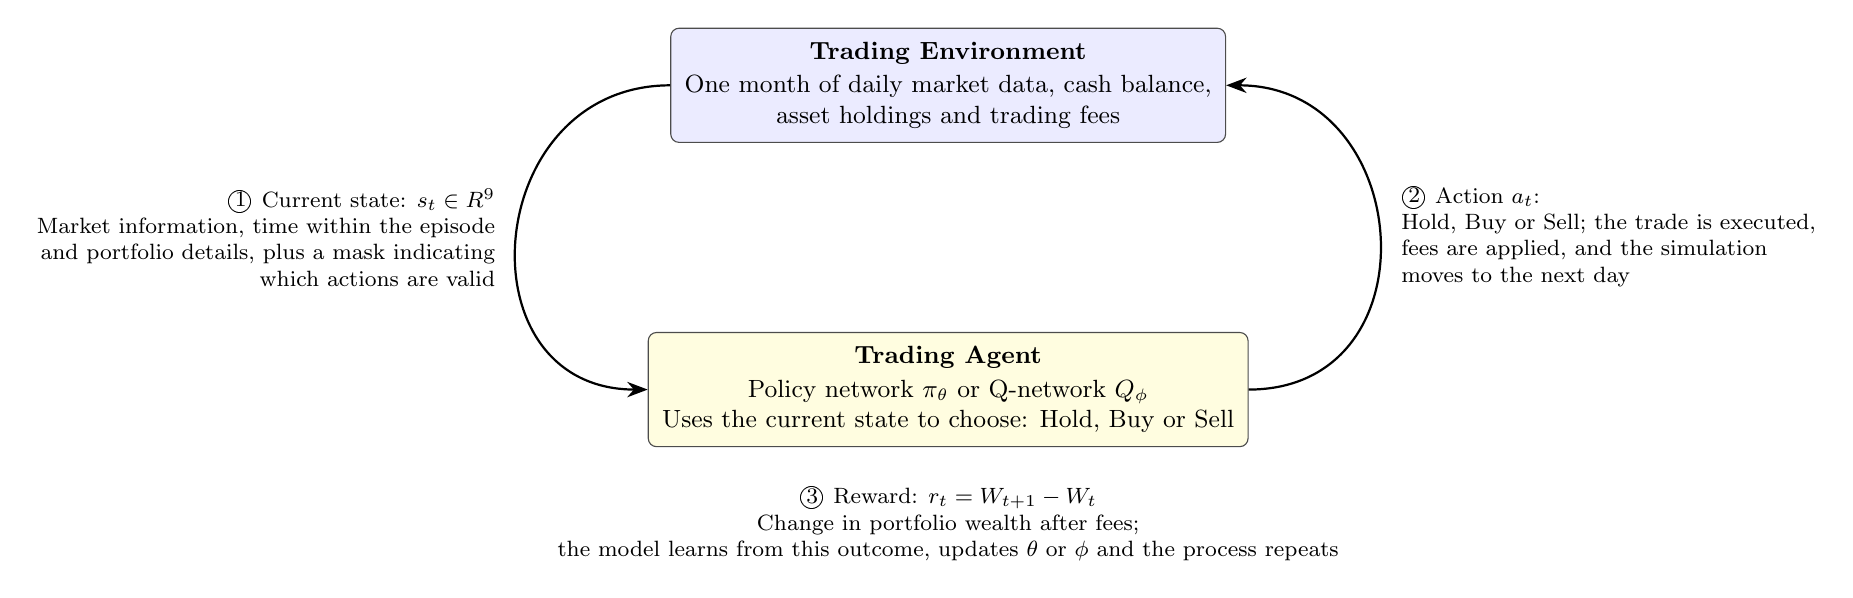
\begin{tikzpicture}[
  box/.style={rectangle, rounded corners=3pt, draw=black!70, align=center,
              minimum width=5.8cm, minimum height=1.45cm, font=\small,
              inner sep=5pt},
  lbl/.style={font=\footnotesize, align=left},
  arr/.style={-{Stealth[length=2.6mm]}, thick}
]
\node[box, fill=blue!8] (env)
  {\textbf{Trading Environment}\\[1pt]
   One month of daily market data, cash balance,\\
   asset holdings and trading fees};

\node[box, fill=yellow!12, below=2.4cm of env] (agent)
  {\textbf{Trading Agent}\\[1pt]
   Policy network $\pi_\theta$ or Q-network $Q_\phi$\\
   Uses the current state to choose: Hold, Buy or Sell};

\draw[arr] (env.west) .. controls +(-2.4,0) and +(-2.4,0) .. (agent.west)
  node[lbl, midway, left=1.5mm, align=right]
  {\textcircled{1} Current state: \mbox{$s_t\in\mathbb{R}^9$}\\
   Market information, time within the episode\\
   and portfolio details, plus a mask indicating\\
   which actions are valid};

\draw[arr] (agent.east) .. controls +(2.4,0) and +(2.4,0) .. (env.east)
  node[lbl, midway, right=1.5mm, align=left]
  {\textcircled{2} Action \mbox{$a_t$}:\\
   Hold, Buy or Sell; the trade is executed,\\
   fees are applied, and the simulation\\
   moves to the next day};

\node[font=\footnotesize, below=0.4cm of agent, align=center]
  {\textcircled{3} Reward: \mbox{$r_t=W_{t+1}-W_t$}\\
   Change in portfolio wealth after fees;\\
   the model learns from this outcome, updates $\theta$ or $\phi$ and the process repeats};
\end{tikzpicture}
\end{document}
